% Options for packages loaded elsewhere
\PassOptionsToPackage{unicode}{hyperref}
\PassOptionsToPackage{hyphens}{url}
%
\documentclass[
  a4paper,
]{article}
\usepackage{amsmath,amssymb}
\usepackage{iftex}
\ifPDFTeX
  \usepackage[T1]{fontenc}
  \usepackage[utf8]{inputenc}
  \usepackage{textcomp} % provide euro and other symbols
\else % if luatex or xetex
  \usepackage{unicode-math} % this also loads fontspec
  \defaultfontfeatures{Scale=MatchLowercase}
  \defaultfontfeatures[\rmfamily]{Ligatures=TeX,Scale=1}
\fi
\usepackage{lmodern}
\ifPDFTeX\else
  % xetex/luatex font selection
\fi
% Use upquote if available, for straight quotes in verbatim environments
\IfFileExists{upquote.sty}{\usepackage{upquote}}{}
\IfFileExists{microtype.sty}{% use microtype if available
  \usepackage[]{microtype}
  \UseMicrotypeSet[protrusion]{basicmath} % disable protrusion for tt fonts
}{}
\makeatletter
\@ifundefined{KOMAClassName}{% if non-KOMA class
  \IfFileExists{parskip.sty}{%
    \usepackage{parskip}
  }{% else
    \setlength{\parindent}{0pt}
    \setlength{\parskip}{6pt plus 2pt minus 1pt}}
}{% if KOMA class
  \KOMAoptions{parskip=half}}
\makeatother
\usepackage{xcolor}
\usepackage[margin=2cm]{geometry}
\usepackage{longtable,booktabs,array}
\usepackage{calc} % for calculating minipage widths
% Correct order of tables after \paragraph or \subparagraph
\usepackage{etoolbox}
\makeatletter
\patchcmd\longtable{\par}{\if@noskipsec\mbox{}\fi\par}{}{}
\makeatother
% Allow footnotes in longtable head/foot
\IfFileExists{footnotehyper.sty}{\usepackage{footnotehyper}}{\usepackage{footnote}}
\makesavenoteenv{longtable}
\usepackage{graphicx}
\makeatletter
\def\maxwidth{\ifdim\Gin@nat@width>\linewidth\linewidth\else\Gin@nat@width\fi}
\def\maxheight{\ifdim\Gin@nat@height>\textheight\textheight\else\Gin@nat@height\fi}
\makeatother
% Scale images if necessary, so that they will not overflow the page
% margins by default, and it is still possible to overwrite the defaults
% using explicit options in \includegraphics[width, height, ...]{}
\setkeys{Gin}{width=\maxwidth,height=\maxheight,keepaspectratio}
% Set default figure placement to htbp
\makeatletter
\def\fps@figure{htbp}
\makeatother
\ifLuaTeX
  \usepackage{luacolor}
  \usepackage[soul]{lua-ul}
\else
  \usepackage{soul}
\fi
\setlength{\emergencystretch}{3em} % prevent overfull lines
\providecommand{\tightlist}{%
  \setlength{\itemsep}{0pt}\setlength{\parskip}{0pt}}
\setcounter{secnumdepth}{-\maxdimen} % remove section numbering
\ifLuaTeX
  \usepackage{selnolig}  % disable illegal ligatures
\fi
\IfFileExists{bookmark.sty}{\usepackage{bookmark}}{\usepackage{hyperref}}
\IfFileExists{xurl.sty}{\usepackage{xurl}}{} % add URL line breaks if available
\urlstyle{same}
\hypersetup{
  pdftitle={DAMSIC},
  pdfauthor={Thomas Debelle},
  hidelinks,
  pdfcreator={LaTeX via pandoc}}

\title{DAMSIC}
\usepackage{etoolbox}
\makeatletter
\providecommand{\subtitle}[1]{% add subtitle to \maketitle
  \apptocmd{\@title}{\par {\large #1 \par}}{}{}
}
\makeatother
\subtitle{\href{https://github.com/Tfloow/Q8_KUL}{An Open-Source
Summary}}
\author{Thomas Debelle}
\date{\today}

\begin{document}
\maketitle

{
\setcounter{tocdepth}{3}
\tableofcontents
}
\hypertarget{sample-hold}{%
\section{Sample \& Hold}\label{sample-hold}}

This summary isn't a perfect 100\(\%\) of the class, it is giving the
broad idea of the class without always going over all the details and
implementation.

\hypertarget{introduction}{%
\subsection{Introduction}\label{introduction}}

Doing analog to digital conversion requires 2 type of discretization :

\begin{enumerate}
\def\labelenumi{\arabic{enumi}.}
\item
  \ul{Time} : sampling
\item
  \ul{Amplitude} : quantization
\end{enumerate}

{adc} to {dac} conversion

r0.5

\begin{figure}
\centering
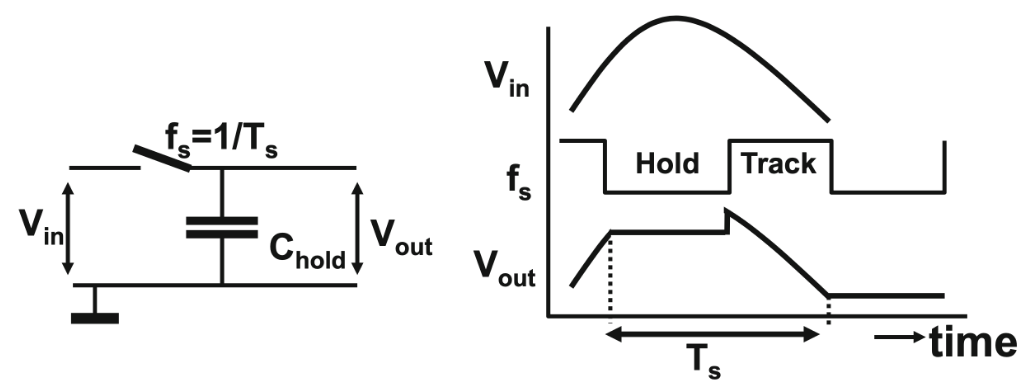
\includegraphics{img/th.png}
\caption{image}
\end{figure}

And of course, going from digital to analog requires to do some
amplitude restoration and holding the signal to make it continuous.
Important to understand that the digital values only make sense if we
have a sampling frequency and a reference voltage where
\(111...111 = V_{ref}\). So the binary number represents a fraction of
this reference voltage.\\
To sample this we are using a \emph{Track and Hold} rather than a sample
and hold since it is not quite easy to sample (opening the switch for a
small small amount of time). Of course, this switch is implemented as a
MOS transistor where we can take advantage of its symmetry to either
charge or discharge the capacitance.\\
If we want to have a \emph{Sample and Hold} we can chain two track and
hold back to back using inverted clocks. But it can be quite tricky to
have such precision when designing the circuit.

\hypertarget{requirements}{%
\paragraph{Requirements}\label{requirements}}

We want good \emph{speed}, so short tracking period and have a high
bandwidth which implies to have a small \(\tau\) (big switch, small
cap). On the other hand, for accuracy we want to have a low noise
(\(\frac{kT}{C}\)) so a big capacitance and low distortion so a linear
switch. We can see this is a major trade-off in T\&H design.

\hypertarget{non-idealities}{%
\subsection{Non-idealities}\label{non-idealities}}

\hypertarget{noise}{%
\subsubsection{Noise}\label{noise}}

r0.33

\begin{figure}
\centering
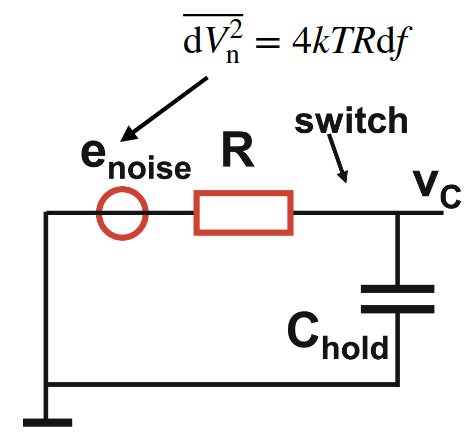
\includegraphics{img/noise_sampling_switch.png}
\caption{image}
\end{figure}

We can represent the switch (implement as a transistor) with a resistor
that has an equivalent noise source \(e_{noise}\). Depending on the
\(C_{hold}\) value we will have various difference equivalent noise
voltages:

\[\begin{aligned}
    v_{C,noise}^2 &= \int_{f=0}^{f=\infty} \frac{4kTR df}{1 + (2\pi f)^2R^2C^2} = \frac{kT}{C}\\
    SNR &= \frac{P_{signal}}{P_{noise}} = \frac{A^2/2}{kT/C}
\end{aligned}\]

Where \(A/\sqrt{2}\) represents the RMS amplitude of the signal. It is
interesting to notice how this noise is only present when we are having
the switch high so theoretically no noise should be present in the hold
phase.\\
Hence, this noise is also sampled ! Even though it will be flat for any
frequency below Shannon and has a zero mean and variance of
\(\sigma = kT/C\). This will create some \emph{aliasing}. The noise PSD
will \textbf{increase} due to sampling since we will have some shorter
bandwidth (\emph{check this}). \[\begin{aligned}
    S_{vv,RC} &= 4kTR = \frac{2kT}{\pi C f_{RC}} & S_{vv,s} &= \frac{2kT}{Cf_s}
\end{aligned}\]

What happens is the fact we have a noise density covering all possible
frequencies which gets sampled and so we have a stack up of noise which
is technically infinite. But since we have a capacitance and resistor
that samples the signal and noise this will act as a low pass filter and
will create some sorts of lobes. The \textbf{total sampled noise} is
always \(kT/C\).\\
The increase of noise spectral density depends on noise bandwidth and
this causes problem for high-resolution converters. It is not always
ideal to have a high bandwidth

\hypertarget{jitter}{%
\subsubsection{Jitter}\label{jitter}}

It is a form of \emph{statistical noise} and is due to noisy clock
generator which won't sample reliably and will sometimes happen slightly
before or after the "\emph{tick}". Jitter can be deterministic which
will result in \emph{tones} in the spectrum or distortion for
signal-dependent jitter (definition of what distortion is). We can find
the result of \(\sigma_t\) has on our sampled amplitude :

\[\begin{aligned}
    A(t) &= A sin(\omega t) & \sigma_A^2(nTs) &= \left(\frac{dA(nTs)}{dt}\right)^2 \sigma_t^2 = \omega^2A^2 cos^2(\omega nT_s)\sigma_t^2\\
    A(nT_s+\Delta t(t)) &= A sin(\omega (nT_s + \Delta t(t)) & \sigma_A^2 &= \frac{\omega^2 A^2 \sigma_t^2}{2}\\ 
    \Delta A(nT_s) &= \frac{d A sin(\omega t)}{dt} \Delta t(nT_s) & \Delta A(nT_s) &=  \omega A cos(\omega nT_S)\Delta t(nT_s) 
\end{aligned}\]

The jitter acts as a sort of ceiling, to fight against the thermal noise
we can simply increase the input voltage but at some point the SNR due
to noise and jitter are equal and the SNR of jitter is the limit since
it only depends on the frequency.

\hypertarget{non-fundamental-error---implementation-error}{%
\subsubsection{Non fundamental error - Implementation
error}\label{non-fundamental-error---implementation-error}}

\hypertarget{pedestal}{%
\paragraph{Pedestal}\label{pedestal}}

Pedestal error is linked with the charges in the channel \textbf{and}
the parasitic cap \(C_{ped}\) which goes from gate to source. There is
some charges that once the switch is closed will get injected or
removed.\\
One solution is the compensation circuit where we will use dummy
switches which will take those extra charges. This requires a duty cycle
of \(50\%\) and precise clock to "capturate" those extra charges
precisely.

\hypertarget{droop}{%
\paragraph{Droop}\label{droop}}

The charges put on \(C_{hold}\) may go down with time especially with
BJT as the base will draw currents. It is linked with leakage :

\[V_{droop} = -\frac{I_{leak} T_{hold}}{C_{hold}}\]

\hypertarget{feedthrough}{%
\paragraph{Feedthrough}\label{feedthrough}}

We also have a capacitance between the source and the drain which will
cause a small current to \emph{feedtrhough}. One solution is to use
\textbf{t-switch} which helps to reduce the effect. In differential
implementations we can use some \emph{cross-coupled always-off}
switches.

\hypertarget{aperture-jitter}{%
\paragraph{Aperture Jitter}\label{aperture-jitter}}

We won't have a perfect instantaneous rise so the logic 1 or logic 0 may
not appear exactly at the clock period.

\hypertarget{capacitor-and-switch-implementations}{%
\subsection{Capacitor and switch
implementations}\label{capacitor-and-switch-implementations}}

\hypertarget{capacitors}{%
\subsubsection{Capacitors}\label{capacitors}}

In IC design we will mostly focus on \textbf{Metal-Insulator-Metal}
(MIM) capacitor which requires a special process and are linear. The
other type is the interconnect \textbf{MOM} which doesn't require a
special process. One key idea is to create the capacitance as high as
possible on the metal layers to get away from parasitic due to the
wafer.\\
We can also do some \emph{vertical} MOM. This solution takes advantage
of the height of the metal stack but the lower end will me more
susceptible to parasitic and we use the other symbol of a capacitance.\\
It is sometimes hard to model capacitance due to the fact we have
multiple field lines going and connecting with all the layers. So one
trick is to isolate each capacitance and shield each one of them. It
makes analysis much easier.

\hypertarget{switches}{%
\subsubsection{Switches}\label{switches}}

The switch (NMOS or PMOS) has its own \(R_{on}\) which is proportional
to \(1/V_{in}\). We not only need a small enough resistor for good
\(\tau\) but also a constant one to avoid distortion !

\[\begin{aligned}
R_{o n, N M O S} & =\frac{1}{(W / L)_N \beta_{N \square}\left(V_{D D}-V_{i n}-V_{T, N}\right)} &
R_{o n, P M O S} & =\frac{1}{(W / L)_P \beta_{P \square}\left(V_{i n}-\left|V_{T, P}\right|\right)}
\end{aligned}\]

One idea to reduce this \(\propto V_{in}\) is to use
\textbf{complementary switches} so the NMOS and PMOS behavior will kinda
cancel out. For this to work we need sufficient \(V_{DD}\) namely
\(V_{DD} < V_{th,n} + |V_{th,p}|\). We can boost V using some
\emph{Cockroft-Walton multiplier} or \emph{Dickson multiplier}.

\hypertarget{bootstrapping}{%
\paragraph{Bootstrapping}\label{bootstrapping}}

The idea behind bootstrapping is to keep the sample pulse and input
voltage constant which will result in constant \(R_{on}\).

\begin{figure}
\hypertarget{fig:enter-label}{%
\centering
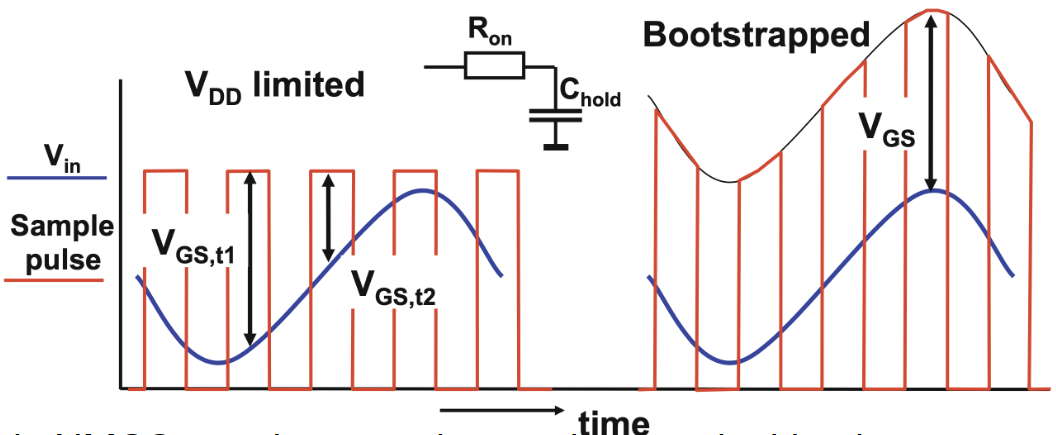
\includegraphics{img/bootstrapping.png}
\caption{Bootstrapping}\label{fig:enter-label}
}
\end{figure}

Here we don't need to use two transistor, we can just use one NMOS and
we get a high SNR for small \(C_{hold}\). We keep the resistance
constant and we don't have any distortion.\\
The main idea is to use a capacitance we charge to \(V_{DD}\) in hold
phase and when the tracking phase come the \(V_{in}\) is added on top of
the \(V_{DD}\) that is stored on the cap making the
\(V_{gs} = V_{DD}\).\\
Some challenges we can face are voltage limit across the gate, drain and
source. We also have a body diode which can create charge lost, latch-up
or even current to substrate.

\begin{figure}
\hypertarget{fig:enter-label}{%
\centering
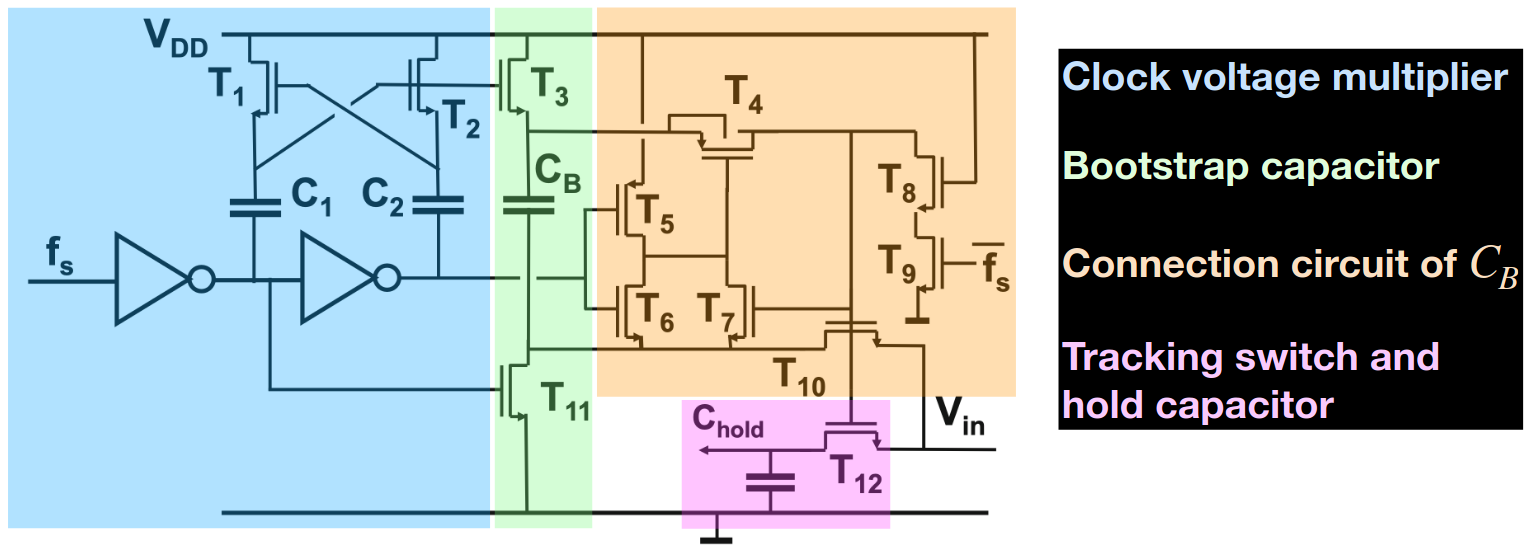
\includegraphics{img/typical_bootstrap.png}
\caption{Typical bootstrap circuit}\label{fig:enter-label}
}
\end{figure}

We can also use a technique called \emph{bottom-plate sampling}. {add
more info read a bit more about it}.

\hypertarget{circuit-topologies}{%
\subsection{Circuit topologies}\label{circuit-topologies}}

\hypertarget{general-considerations}{%
\subsubsection{General considerations}\label{general-considerations}}

We want to maintain the value on the capacitance, one solution is to use
buffered implementation. Buffered implementation will be more accurate
but we introduce a feedback system which inherently has delay thus some
maximum possible speed.\\
We also need to keep in mind that when using a buffer (opamp) we will
have an extra \emph{non-linear} capacitance in parallel with our hold
capacitance. So we need to pick the right hold capacitance to minimize
this extra non linear capacitance.\\
We always need to keep in mind what is this designed use for, what is
the swing (rail-to-rail, buffer supply voltage above \(V_{DD}\), ...).\\
High-gain opamp requires a low settling error
\(A_{DC} > \frac{1}{\epsilon} = 2^N\). The settling speed determnies
unity-gain frequency of a track and hold buffer. the UGF palys a big
role.

\hypertarget{switched-capacitor-t-h-circuits}{%
\subsubsection{Switched-capacitor T\& H
circuits}\label{switched-capacitor-t-h-circuits}}

The most basic switched-cap implementation :

\begin{figure}
\hypertarget{fig:basic-sc-label}{%
\centering
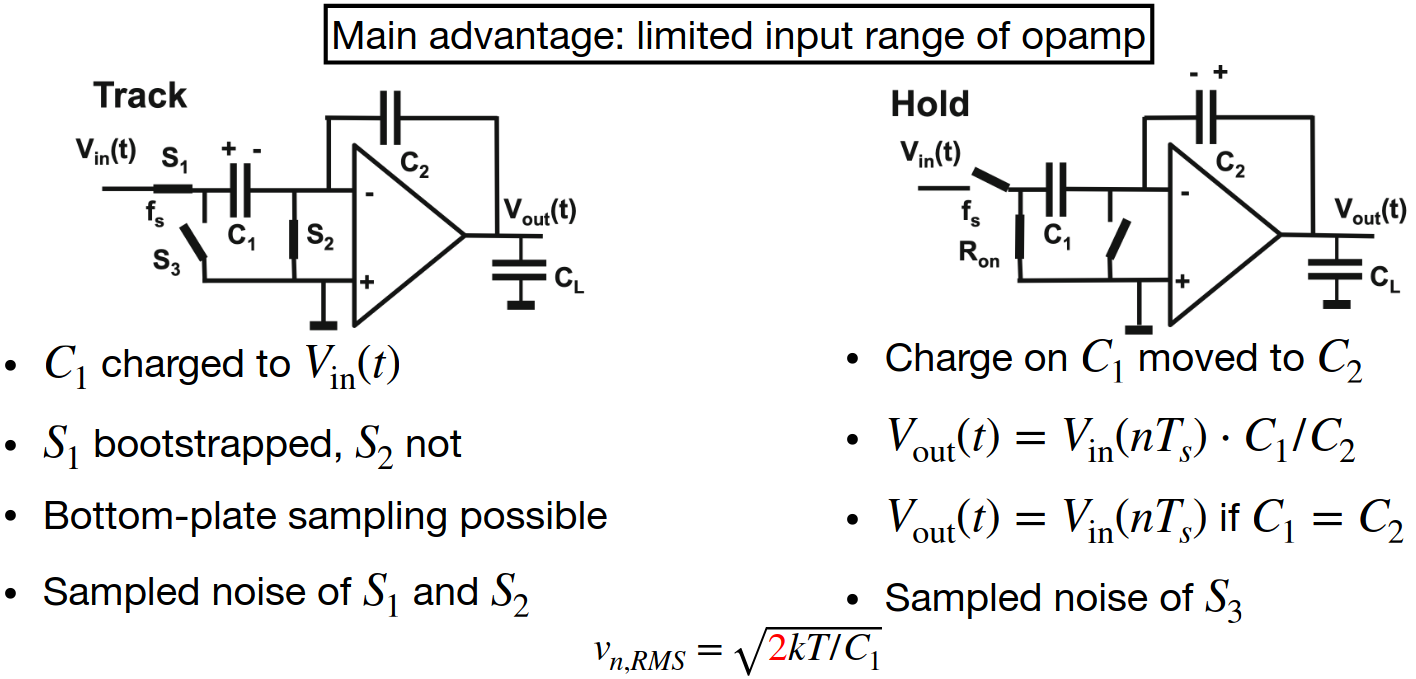
\includegraphics{img/basic_th_switched_cap.png}
\caption{Basic Switched-cap implementation}\label{fig:basic-sc-label}
}
\end{figure}

In the \emph{track phase} we first discharge \(C_2\). The \(S_1\) is
\emph{bootstrapped} and \(C_1\) is charged to \(V_{in}\). We have some
sampled noise at \(S_1\) and \(S_2\). In the \emph{hold phase}, the
charge from \(C_1\) are moved to \(C_2\) (charge recollection). We have
\(V_{out}(t) = V_{in}(nT_S) \cdot C1/C2\).\\
If we have \emph{unity-gain signal} we will have a
\(H = C_2/(C_1+C_2) = 1/2\) if \(C_1 = C_2\). The closed loop gain is
\(A_{cl} = 2\) so we will amplify some unwanted signal. The setting time
is determined by \(1/2 \tau\).

\hypertarget{flip-around-th}{%
\subsubsection{Flip-Around T\&H}\label{flip-around-th}}

\begin{figure}
\hypertarget{fig:flip-around-label}{%
\centering
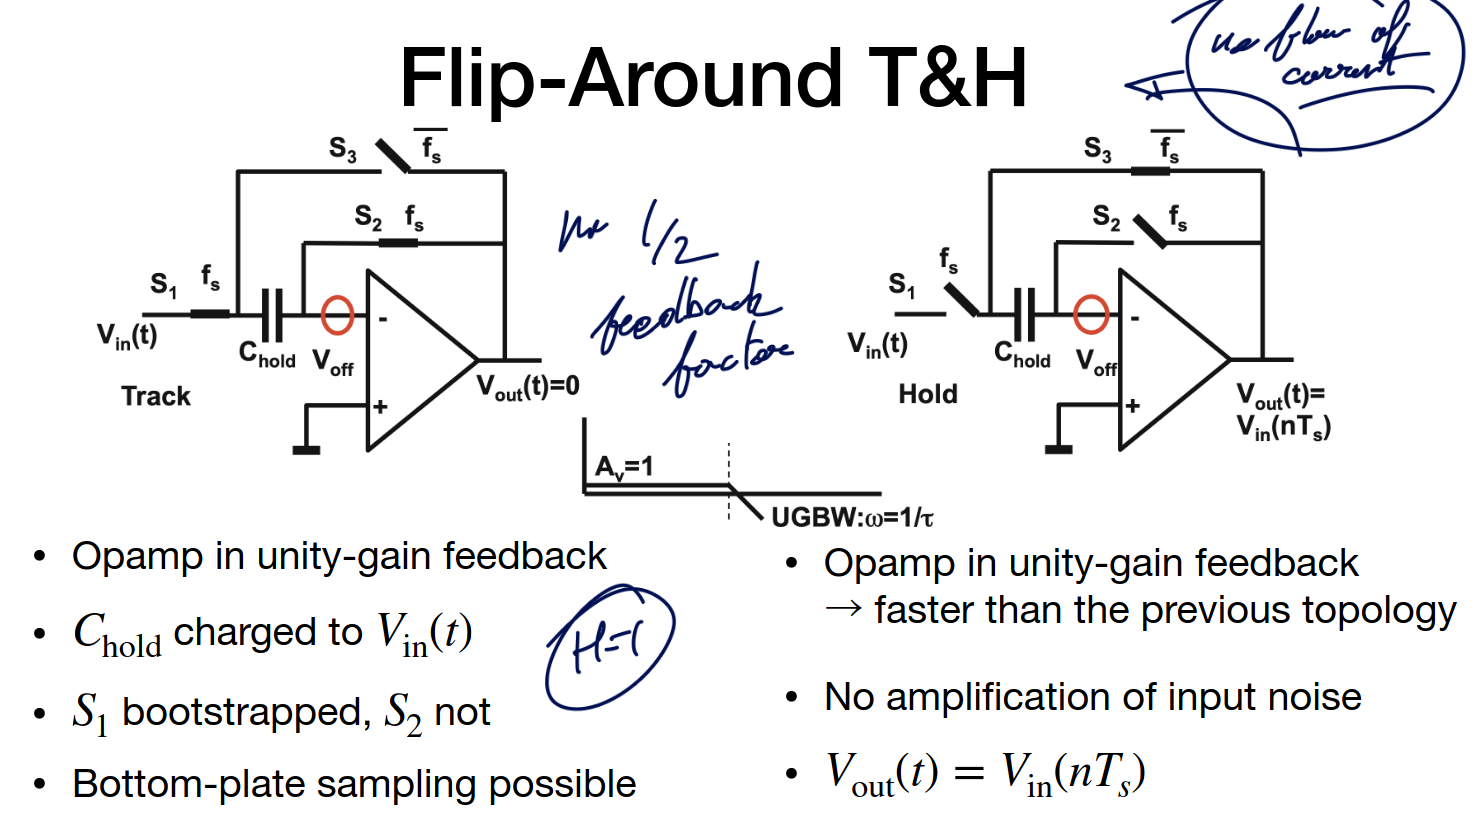
\includegraphics{img/Flip_around.png}
\caption{Flip-Around track \& hold}\label{fig:flip-around-label}
}
\end{figure}

It will use a virtual ground to charge and discharge the cap. Here we
have a unity-gain feedback of 1 which is desirable. But this virtual
ground isn't perfect and so we will have some \emph{offset}. But this
offset will actually be cancelled !

\[\begin{aligned}
    \text{Track mode : }& V_{C_{hold}} (nT_S) = V_{in}(nT_S) - V_{off} \\
    \text{Hold mode : }&  V_{out}((n+1/2)T_S) = V_{C_{hold}} (nT_S) + V_{off} = V_{in}(nT_S)
\end{aligned}\]

If we go in the z-domain to analyze this error we find :

\[\begin{aligned}
    V_{out,error} &= V_{off} (z) (1-z^{-0.5})\\
    H(f) &= 2 sin(\pi f/2f_s)
\end{aligned}\]

So it will suppress the offset and the noise at low-frequency. But the
high-frequency noise will be doubled and the sample noise on
\(C_{hold}\) is still present.

\begin{figure}
\hypertarget{fig:amplifying-th-label}{%
\centering
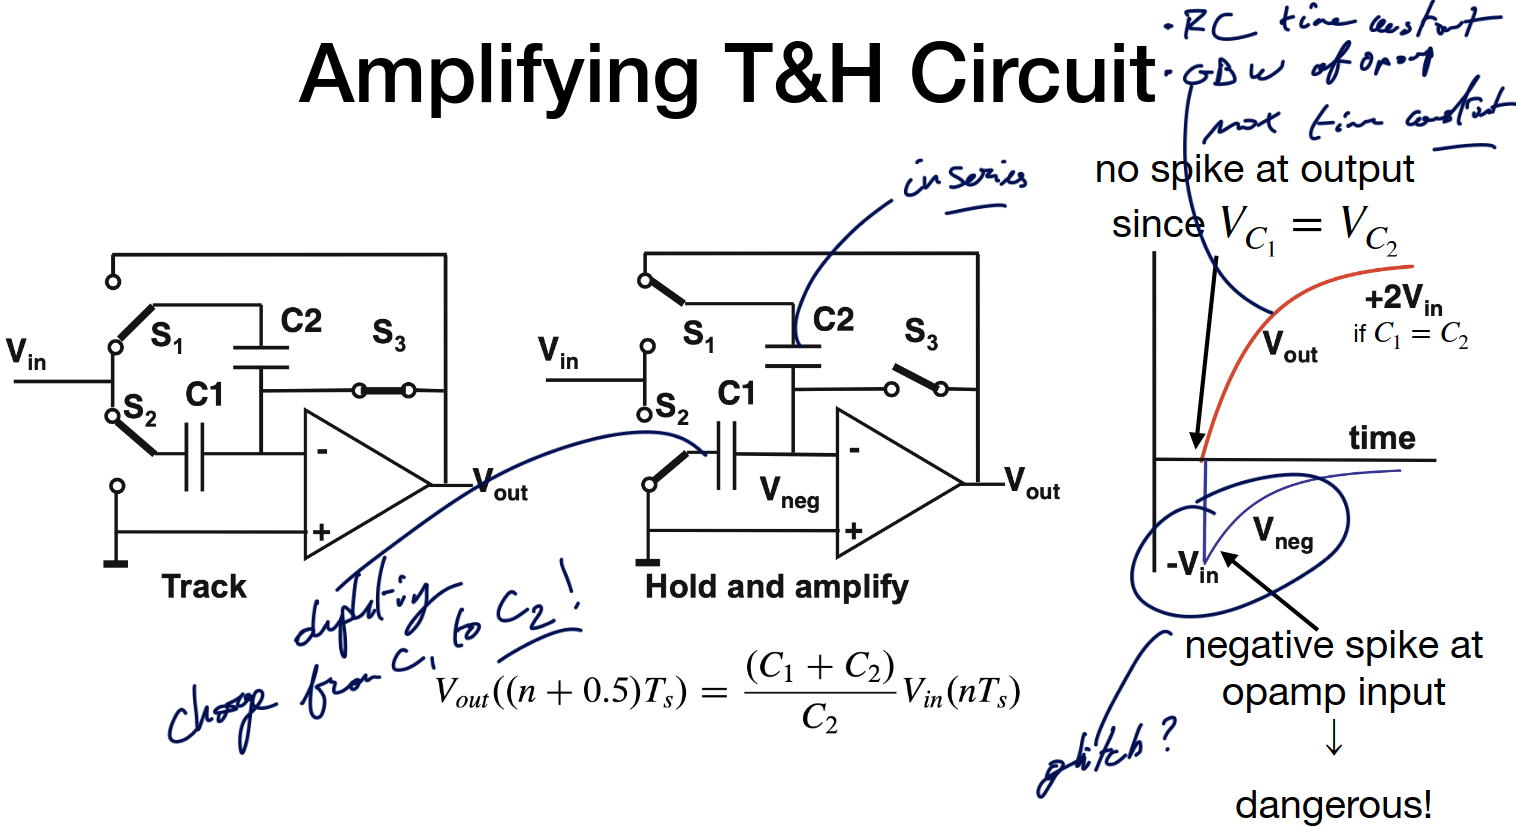
\includegraphics{img/Amplifying_Track.png}
\caption{Amplifying track \& hold}\label{fig:amplifying-th-label}
}
\end{figure}

We can see some dangerous spikes on fig.
\protect\hyperlink{fig:amplifying-th-label}{1.5}. The noise can be found
as follow :

\[\begin{aligned}
    v_{in,noise}^2 &= \frac{kT}{C_1+C_2} & v_{out,noise}^2 &= \frac{kT(C_1+C_2)}{C_2^2} + \text{noise OpAmp}
\end{aligned}\]

\hypertarget{correlated-double-sampling}{%
\subsubsection{Correlated double
sampling}\label{correlated-double-sampling}}

In sensors and and image sensor we want to get rid of those unwanted
component. Often, we will have 2 samples time where we will first get a
baseline then the actual signal we want to remove the offset component.

\begin{figure}
\hypertarget{fig:double-correlated-label}{%
\centering
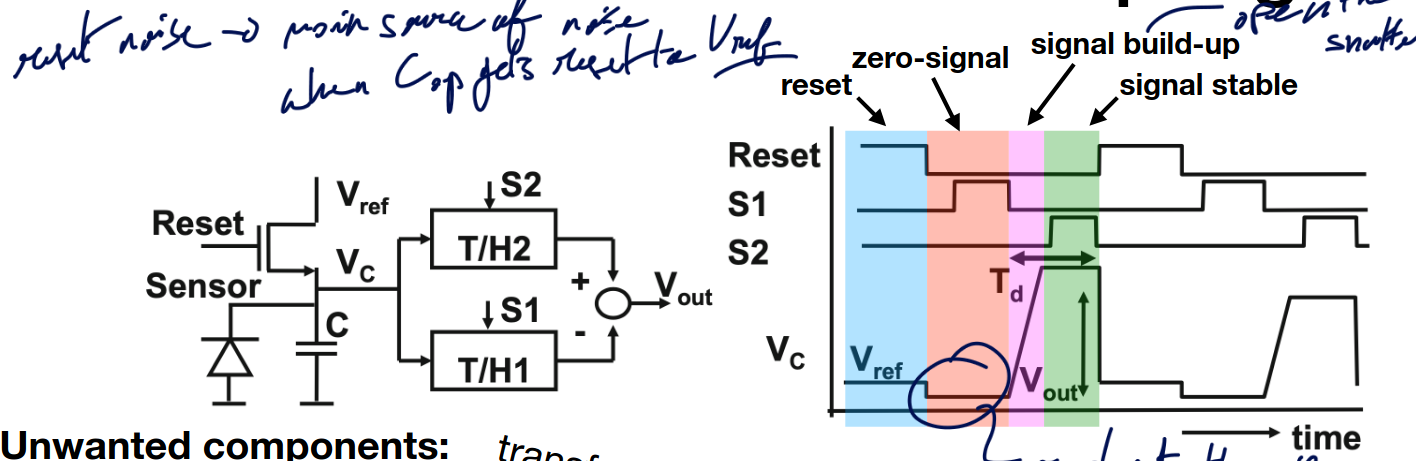
\includegraphics{img/double_corr.png}
\caption{Correlated double sampling}\label{fig:double-correlated-label}
}
\end{figure}

\[\begin{aligned}
    |H(s)| &= |1 - e^{-sT_d}| = |e^{-sTd/2}| = |e^{-sT_d /2} 2 sin(sT_d /2) |\\
    |H(\omega)| &= |2sin(\omega T_d / 2)| = |2 sin(\pi f T_d)|
\end{aligned}\]

It will reject the low-frequency noise but will \emph{amplify} by
\(1/2T_d\) the noise near \emph{odd multiples}.

\hypertarget{digital-to-analog-conversion}{%
\section{Digital-to-Analog
Conversion}\label{digital-to-analog-conversion}}

We need to differentiate two different use cases of a {dac} namely :

\begin{enumerate}
\def\labelenumi{\arabic{enumi}.}
\item
  \ul{Convert to physical domain :} when we need a \emph{high quality}
  at every time instant. We need a minimum amount of power to be able to
  draw some current. For example a USB-C to jack adapter !
\item
  \ul{Generate reference value for an {adc} :} typically needed in a SAR
  {adc}. We only need this conversion at some specific point in time and
  the drive capabilities are not exigent.
\end{enumerate}

\hypertarget{signal-representations}{%
\subsection{Signal representations}\label{signal-representations}}

\begin{itemize}
\item
  \ul{Straight binary:} only positive signals
\item
  \ul{Two's complement:} easy addition and subtraction, zero signal at
  half reference (noisy!)
\item
  \ul{Sign and magnitude:} no noisy half reference values for zero
  signal, digital decoder needed, simple rounding results in cross-over
  distortion
\item
  \ul{Gray coded:} only one bit changes
\end{itemize}

\hypertarget{tab:binary}{}
\begin{longtable}[]{@{}clclclcl@{}}
\caption{Binary Representations}\tabularnewline
\toprule\noalign{}
\textbf{Straight binary} & & \textbf{Two's complement} & &
\textbf{Sign+magnitude} & & \textbf{Gray coded} & \\
\midrule\noalign{}
\endfirsthead
\toprule\noalign{}
\textbf{Straight binary} & & \textbf{Two's complement} & &
\textbf{Sign+magnitude} & & \textbf{Gray coded} & \\
\midrule\noalign{}
\endhead
\bottomrule\noalign{}
\endlastfoot
15 & 1111 & 7 & 0111 & 7 & 0111 & 15 & 1000 \\
14 & 1110 & 6 & 0110 & 6 & 0110 & 14 & 1001 \\
13 & 1101 & 5 & 0101 & 5 & 0101 & 13 & 1011 \\
12 & 1100 & 4 & 0100 & 4 & 0100 & 12 & 1010 \\
11 & 1011 & 3 & 0011 & 3 & 0011 & 11 & 1110 \\
10 & 1010 & 2 & 0010 & 2 & 0010 & 10 & 1111 \\
9 & 1001 & 1 & 0001 & 1 & 0001 & 9 & 1101 \\
8 & 1000 & 0 & 0000 & 0 & 0000 & 8 & 1100 \\
7 & 0111 & -1 & 1111 & 0 & 1000 & 7 & 0100 \\
6 & 0110 & -2 & 1110 & -1 & 1001 & 6 & 0101 \\
5 & 0101 & -3 & 1101 & -2 & 1010 & 5 & 0111 \\
4 & 0100 & -4 & 1100 & -3 & 1011 & 4 & 0110 \\
3 & 0011 & -5 & 1011 & -4 & 1100 & 3 & 0010 \\
2 & 0010 & -6 & 1010 & -5 & 1101 & 2 & 0011 \\
1 & 0001 & -7 & 1001 & -6 & 1110 & 1 & 0001 \\
0 & 0000 & -8 & 1000 & -7 & 1111 & 0 & 0000 \\
\end{longtable}

To represent those bits in hardware we can go either for the
\emph{thermometer} or \emph{binary} representation. In the thermometer
representation each cells are of the same size and to increase numbers
we need to increase the amount of cells on. It grantees
\textbf{monotonicity}. For the binary, they are not of equal size but
has the advantage to need \(n\) for \(n\) bits while it is \(2^n\) cells
for thermometer. It is not guaranteed to be monotonic and the large
switch of cells can create glitches.\\
We can also use \emph{segmentation} to leverage from both type of
implementation.

\hypertarget{tab:unary_vs_binary}{}
\begin{longtable}[]{@{}lcc@{}}
\caption{Comparison between Unary and Binary
Architectures}\tabularnewline
\toprule\noalign{}
\textbf{Architecture} & \textbf{Unary} & \textbf{Binary} \\
\midrule\noalign{}
\endfirsthead
\toprule\noalign{}
\textbf{Architecture} & \textbf{Unary} & \textbf{Binary} \\
\midrule\noalign{}
\endhead
\bottomrule\noalign{}
\endlastfoot
Monotonicity & By design & Not guaranteed \\
Number of elements & \(\propto 2^N\) & \(\propto N\) \\
Area, parasitics & \(\propto 2^N\) & \(\propto N\) \\
{inl} systematic & Gradient & Small \\
{inl} random & \(\propto \sigma_{element} \sqrt{2^N-1}\) & Same with
{dnl} errors \\
{dnl} random & \(\propto \sigma_{element}\) &
\(\propto \sigma_{element} \sqrt{N, \dots, 2^N-1}\) \\
Switching energy & \(\propto\) Signal & Can be large and non-linear \\
Decoder complexity & \(2^N\)-to-1 & Simple \\
Power & Choice for R, I, or C implementation dominates power & \\
Noise & Similar for similar power levels & \\
\end{longtable}

We need to keep in mind that the {dnl} is the difference between one
step to the other and it must be lower than \(1 LSB\). The {inl} is the
integrate error and so cumulate the error. Those issues will lead to
distortion and harmonics !

\hypertarget{typical-inl-of-unary-architectures}{%
\subsubsection{\texorpdfstring{Typical {inl} of Unary
Architectures}{Typical inl of Unary Architectures}}\label{typical-inl-of-unary-architectures}}

Here we have \(A_{lsb}\) that represents the minimum voltage we can add
so the minimum cell. To represents a number and it's unused counter part
:

\[\begin{aligned}
    y_1 &= \sum_{i=0}^{m-1} A_{lsb}(i) \quad \mathbb{E}(y_1) = m A_{lsb} \quad \sigma_{y_1} = \sigma_{A_{lsb}} \sqrt{m}\\
    y_2 &= \sum_{i=m}^{2^N-1} A_{lsb}(i) \quad \mathbb{E}(y_2) = (2^N-m) A_{lsb} \quad \sigma_{y_2} = \sigma_{A_{lsb}} \sqrt{2^N -m}
\end{aligned}\]

To find the {inl} we can use this formula \textbf{WHY THIS FORMULA I
DON4T GET IT ???}

\[\begin{aligned}
    INL(m) &= \frac{2^N \sum_{i=0}^{m-1} A_{lsb}(i) }{\sum_{i=0}^{2^N - 1} A_{lsb}(i) } - m = \frac{2^N y_1}{y_1 + y_2}  - m\\
    \sigma_{INL}^2(m) &= \left(\frac{\partial INL(m)}{\partial y_1} \right)^2 \sigma_{y_1}^2 + \left(\frac{\partial INL(m)}{\partial y_2} \right)^2 \sigma_{y_2}^2\\
    &= \left( \frac{y_2}{(y_1+y_2)^2} \right)^2 m \sigma_{A_{lsb}}^2 + \left( \frac{-y_1}{(y_1+y_2)^2} \right)^2 (2^N-m) \sigma_{A_{lsb}}^2\\
    &= \frac{m(2^N - m)}{2^N} \frac{\sigma_{A_{lsb}}}{A_{lsb}^2}
\end{aligned}\]

\hypertarget{segmented-cells}{%
\paragraph{Segmented cells}\label{segmented-cells}}

\begin{figure}
\hypertarget{fig:segmented-cell-label}{%
\centering
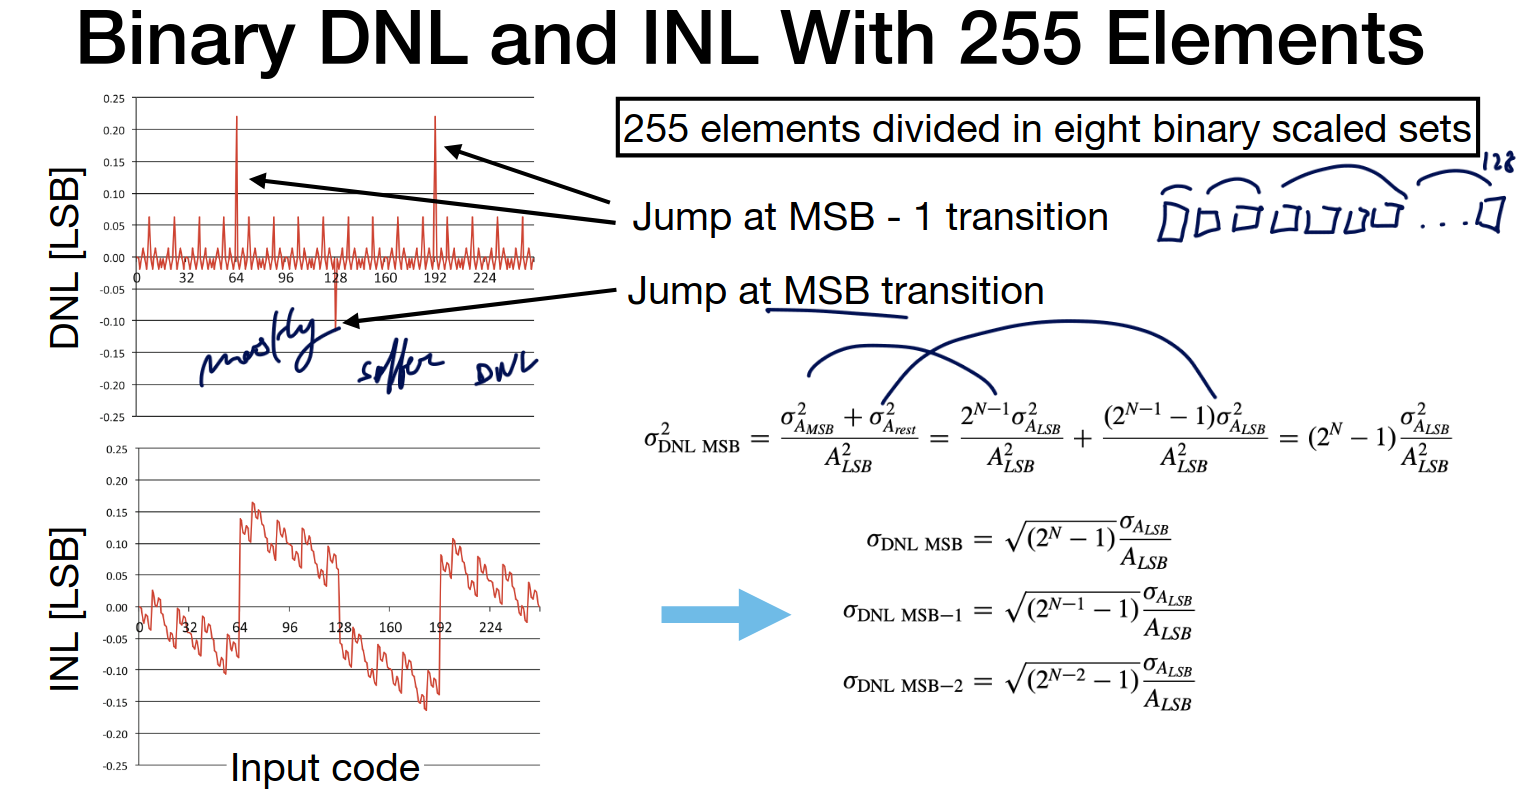
\includegraphics{img/segmented_DNL_INL.png}
\caption{Segmented {dnl} and {inl}}\label{fig:segmented-cell-label}
}
\end{figure}

The less binary scaled elements we have the stronger those jumps and
glitches will be. It may even lead to {dnl} being over \(1\) LSB meaning
we can't guarantee monotonicity anymore this will result in missing
code.

\[\sigma_{DNL, MSB} = (2^N -1) \frac{\sigma_{A_{lsb}}}{A_{lsb}}\]

\hypertarget{tab:unary_binary_comparison}{}
\begin{longtable}[]{@{}lcc@{}}
\caption{Comparison of Unary and Binary Architectures, {dac} and
{adc}}\tabularnewline
\toprule\noalign{}
& \textbf{Unary} & \textbf{Binary} \\
\midrule\noalign{}
\endfirsthead
\toprule\noalign{}
& \textbf{Unary} & \textbf{Binary} \\
\midrule\noalign{}
\endhead
\bottomrule\noalign{}
\endlastfoot
Voltage & Resistor string & R-2R \\
& \emph{Flash {adc}} & \emph{Low-performance {dac}} \\
Current & Current matrix & Current splitting \\
& \emph{High bandwidth {dac}} & \\
Charge/capacitor & Capacitor bank & Capacitor bank \\
& \emph{Low power {dac}} & \\
Time & PWM, \(\Sigma\Delta\) mod & Limited by distortion \\
& \emph{Low bandwidth {dac}} & \\
\end{longtable}

\hypertarget{digital-to-analog-conversion-1}{%
\subsection{Digital-to-analog
conversion}\label{digital-to-analog-conversion-1}}

\hypertarget{voltage-domain}{%
\subsubsection{Voltage domain}\label{voltage-domain}}

\hypertarget{resistor-ladder}{%
\paragraph{Resistor ladder}\label{resistor-ladder}}

The simplest {dac} we can think of is a \textbf{resistive ladder} where
we use a thermometer code based approach. We need \(2^N\) resistors
between \(V_{ref+}\) and \(V_{ref-}\). We need a buffer to drive the
load so we don't have some currents that flow back into the resistive
ladder which would cause some monoticity and values change. This buffer
op-amp isn't straightforward as it needs to be a rail-to-rail op-amp.\\
The equivalent input impedance seen by the input of the buffer is given
as :

\[R_{eq} (m) = \frac{\frac{m}{2^N} R_{tot} \cdot \frac{2^N-m}{2^N} R_{tot} }{\frac{m}{2^N} R_{tot} + \frac{2^N-m}{2^N} R_{tot}} = \frac{m(2^N-m)}{2^{N+1}} R_{tot}\]

We have a signal-dependent current delivery and the resistor is
parabolic. Due to the capacitive load we also have a signal-dependent
time constant. This lead to distortion at high frequencies.

\[\begin{aligned}
    V(m) &= \frac{m}{2^N} V_{ref} = \frac{mR}{mR + (2^N -m)R} V_{ref} = \frac{R_1}{R_1 + R_2} V_{ref}\\
    \sigma_{V}^2(m) &= \left( \frac{\partial V(m)}{\partial R_1} \right)^2 \sigma_{R_1}^2  + \left( \frac{\partial V(m)}{\partial R_2} \right)^2 \sigma_{R_2}^2 \\
    &= \left( \frac{R_2}{(R_1+R_2)^2} \right)^2 \sigma_{R_1}^2 V_{ref}^2  +  \left( \frac{-R_1}{(R_1+R_2)^2} \right)^2 \sigma_{R_2}^2 V_{ref}^2\\
    &= \frac{m(2^N -m)}{2^N} \frac{\sigma_R^2}{R^2} \frac{V_{ref}^2}{2^{2N}} =  \frac{m(2^N -m)}{2^N} \frac{\sigma_R^2}{R^2} V_{LSB}^2\\ 
    \sigma_{INL}^2 &= \frac{m(2^N- m)}{2^N} \frac{\sigma_R^2}{R^2}
\end{aligned}\]

\textbf{ADD MORE INFO}

\hypertarget{r-2r-ladder}{%
\paragraph{R-2R ladder}\label{r-2r-ladder}}

\begin{figure}
\hypertarget{fig:R-2R-label}{%
\centering
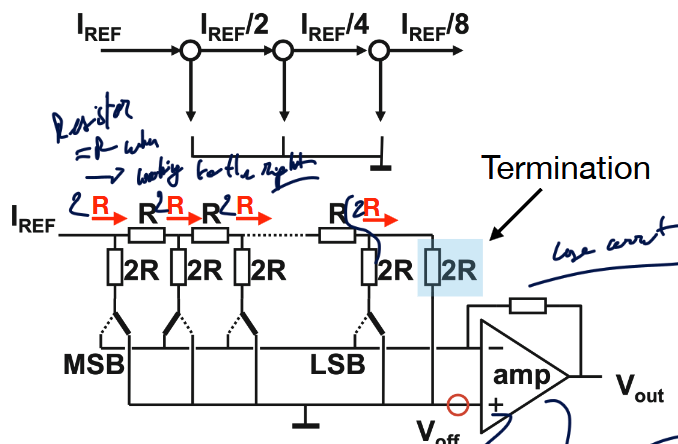
\includegraphics{img/R_2R.png}
\caption{R-2R Ladders}\label{fig:R-2R-label}
}
\end{figure}

Here we are using a binary structure and we only need a \(2N\)
resistors. It is not super precise since we have a lower and lower
current flowing in each branch which will be more susceptible to noise.
The accuracy depends on :

\begin{enumerate}
\def\labelenumi{\arabic{enumi}.}
\item
  \ul{Offset voltage :} non-ideal virtual ground and so we have some
  error in the current split. \(V_{off} < \frac{I_{REF} R}{2^N}\).
\item
  \ul{Resistor matching :} we need good matching or we will have large
  difference.
\item
  \ul{Switch resistance :} the switch will add some \(R_{on}\)
  resistance so we need it to be small to have a small impact.
\end{enumerate}

\hypertarget{segmented-resistor-ladder}{%
\paragraph{Segmented resistor ladder}\label{segmented-resistor-ladder}}

\begin{figure}
\hypertarget{fig:segmented-resistor-label}{%
\centering
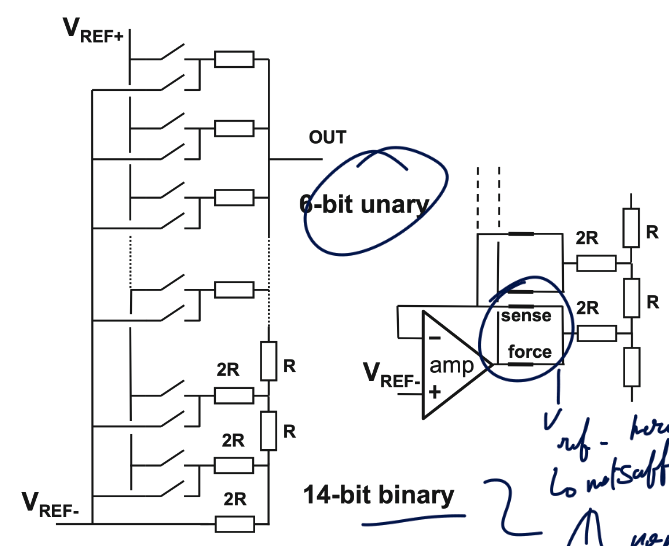
\includegraphics{img/segmented_r_ladder.png}
\caption{Segmented resistor ladder}\label{fig:segmented-resistor-label}
}
\end{figure}

We will have a thermometer and binary part. It will improve the
precision. There is no current in sense path. The sense node is equal to
\(V_{ref}\). We calibrate this offset voltage and we can also call it a
\emph{kelvin contact} or \emph{four-point sensing}.

\hypertarget{current-domain}{%
\subsubsection{Current domain}\label{current-domain}}

Here instead of using resistor that will drive another resistor creating
a voltage that gets buffered, we will directly work with current source
that will drive a resistor which will have its voltage buffered. We can
either go for a thermometer or binary coded version :

\begin{figure}
\hypertarget{fig:enter-label}{%
\centering
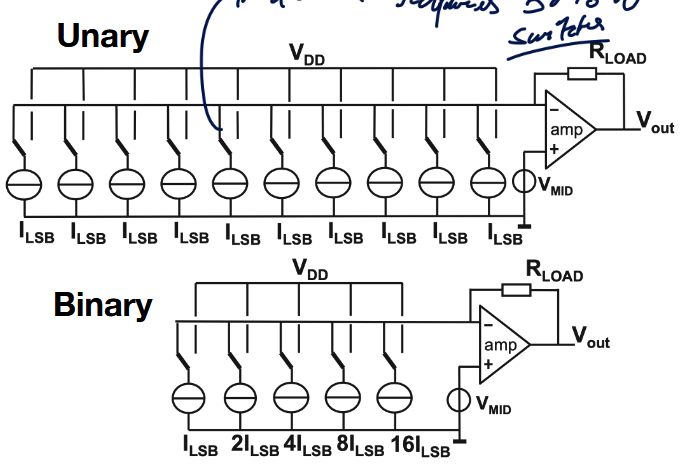
\includegraphics{img/Buffered_Current_DAC.png}
\caption{Buffered Current {dac}}\label{fig:enter-label}
}
\end{figure}

We need to keep all current source on even if they are not used to avoid
\emph{current dump}. The amplifier is sensing the current so we call it
a {tia}. We need a low input impedance to limit the swing and low output
one so we can drive any type of load.

\hypertarget{symmetrical-buffered-current-dac}{%
\paragraph{Symmetrical Buffered
current-DAC}\label{symmetrical-buffered-current-dac}}

\begin{figure}
\hypertarget{fig:sym-buffered-DAC-label}{%
\centering
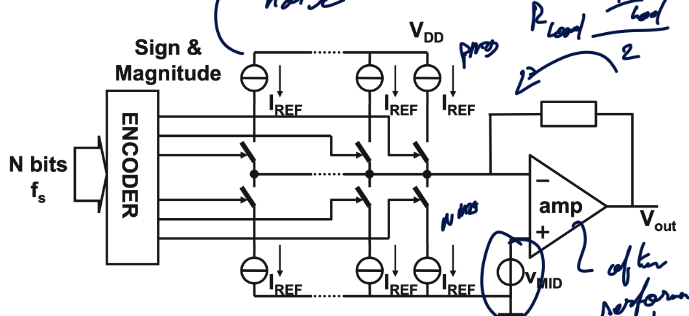
\includegraphics{img/sym_dac.png}
\caption{Symmetrical buffered
current-DAC}\label{fig:sym-buffered-DAC-label}
}
\end{figure}

To avoid some important switching (on and off) due to the representation
of a number in signed format, we want to use a symmetrical one. Since
most of the signal will be around 0 often going positive and negative.
This configuration will reduce the 1/f and thermal noise. Here we need a
current sink and current source so a NMOS and PMOS network is required
(may be a designed constraint and we need to match PMOS and NMOS). We
only have the noise of the buffer for zero level. We will need some
calibration to manage a balance between NMOS and PMOS.

\hypertarget{buffer-less-current-dac}{%
\paragraph{Buffer-less current-DAC}\label{buffer-less-current-dac}}

\begin{figure}
\hypertarget{fig:BLC-DAC-label}{%
\centering
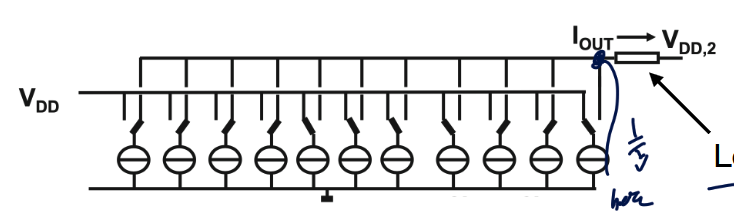
\includegraphics{img/bufferless_current_dac.png}
\caption{Buffer-less Current DAC}\label{fig:BLC-DAC-label}
}
\end{figure}

Since we are not using a buffer, we have theoretically a larger
bandwidth since we are not limited by the spec of a {tia}. But in life
there is always parasitic and so we will have a pole determined by the
output load impedance and capacitance. It is a good choice for
time-continuous signals with a matched impedance between
\(50-75\Omega\).

\hypertarget{segment-current-dac}{%
\paragraph{Segment current DAC}\label{segment-current-dac}}

Based on the same idea of a buffer-less DAC we can use some current
source that are \(2^a\) LSB and some binary based sources starting at 1.
This is segmenting and we use the thermometer for MSB part and the
binary for the LSB as they take less space. The biggest issue is when we
switch off binary section and we switch to the next unary source :

\begin{figure}
\centering
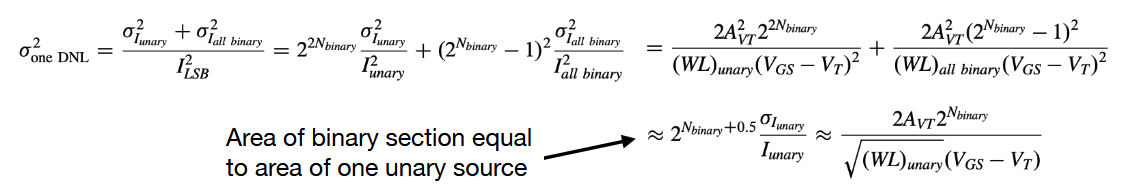
\includegraphics{eq_segme.png}
\caption{image}
\end{figure}

We can also go further and add an extra rail to create current divider.
This third rail will \emph{steer} unary current to current divider. The
divider can be unary or binary scaled but we will have large transition
error at the edge that will be reduced.

\hypertarget{matrix-decoding}{%
\paragraph{Matrix decoding}\label{matrix-decoding}}

r0.5 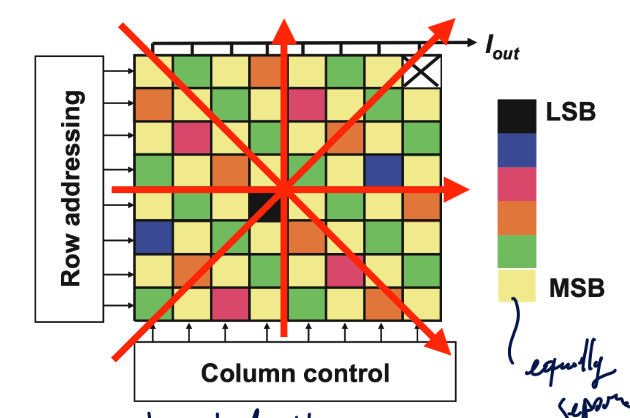
\includegraphics{img/centroid_layout.png}

Usually in VLSI we will arrange thermometer current source in a matrix
format so we can simply and quickly access the current. But due to the
spreading of those current sources, we will accentuate some physical
phenomena such as \emph{oxide thickness, power delivery drop, clock
timing, temperature, ...} which will make the current sources unequal.\\
One technique to reduce this effect is presented on figure
\protect\hyperlink{fig:centroid-layout-label}{{[}fig:centroid-layout-label{]}}.
We create symmetry in both direction and we will get rid of any
\textbf{linear gradient}. We can go even further with some \(Q^2\) walk
and distributed subcell across the complete array or even use some
\emph{randomize current cell} from one sample to the next (more
advanced).\\
Some calibration we can make is \textbf{current source sorting} where we
will measure all of the cells and create a sort of pair where we trigger
a larger cell with a smaller one after. But we need a lot of
pre-processing and measurements and we need to create some special metal
routing over the cells which can deteriorate the performances even more.
We also need into account possible delay and timing issues, ...

\hypertarget{current-cell-implementation}{%
\paragraph{Current cell
implementation}\label{current-cell-implementation}}

r0.5 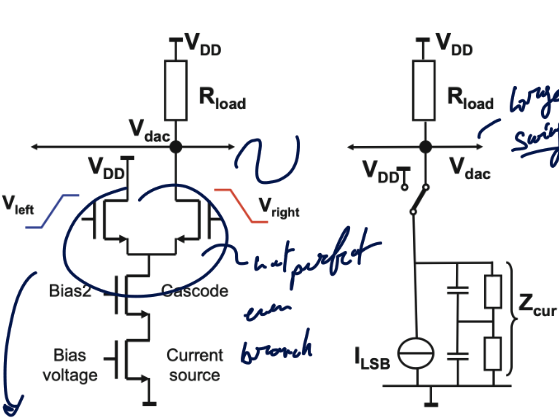
\includegraphics{img/current_cell.png}

We keep the current source on to avoid distortion and keep the power
consumption constant. The \(V_{dac}\) will have considerable voltage
variation which will create distortion.\\
Ideally the voltage drop is :

\[\begin{aligned}
    V_{DD} - V_{dac} &= \alpha 2^N I_{LSB} R_{load}\\
    I_{err} &= \alpha Z^N V_{dac} / |Z_{cur}|
\end{aligned}\]

But we have a real voltage drop of :

\[\begin{aligned}
    V_{DD} - V_{dac} &= R_{load} \left( \alpha 2^N I_{LSB} + \frac{\alpha 2^N V_{dac}}{|Z_{cur}|} \right)
\end{aligned}\] \[\begin{aligned}
    V_{dac} &= \frac{V_{DD} - R_{load} \alpha 2^N I_{LSB}}{1 + \alpha 2^N R_{load} / |Z_{cur}|}\\
    &\approx (V_{DD} - R_{load} \alpha 2^N I_{LSB}) \left( 1- \frac{\alpha 2^N R_{load}}{|Z_{cur}|}  + \left( \frac{\alpha 2^N R_{load}}{|Z_{cur}|} \right)^2 \right)
\end{aligned}\]

We will have a HD3 with \(((2^N R_{load})/(4|Z_{cur}|))^2\)

\hypertarget{switch-implementation}{%
\paragraph{Switch implementation}\label{switch-implementation}}

r0.3 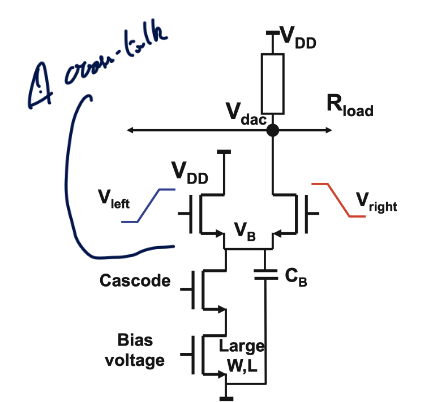
\includegraphics{img/switch_impl.png}

Switches are controlled by low-swing differential pulses to reduce
cross-talk and minimize the creation of an inversion charge. We need to
minimize the \(V_B\) to have extremely accurate timing of switches.
There is some charge taken from or released in output node at every
switching event. Glitches are problematic for time-continuous output.\\
Architecture of choice for most demanding applications. We have a
constant (high) power consumption and need a high-frequency clock and
decoding logic require significant power. Differential implementation to
cancel second-order distortion (big advantage). First-order relationship
between linearity and bandwidth.

\hypertarget{charge-domain}{%
\subsubsection{Charge domain}\label{charge-domain}}

\hypertarget{time-domain}{%
\subsubsection{Time domain}\label{time-domain}}

\hypertarget{accuracy-improvement-methods}{%
\subsection{Accuracy improvement
methods}\label{accuracy-improvement-methods}}

\hypertarget{nyquist-adc}{%
\section{Nyquist ADC}\label{nyquist-adc}}

This chapter will focus essentially about the comparator and will only
cover some techniques applicable to Nyquist ADC.

\hypertarget{comparator}{%
\subsection{Comparator}\label{comparator}}

\hypertarget{comparator-1}{%
\subsection{Comparator}\label{comparator-1}}

\hypertarget{requirements-and-operation-principle}{%
\subsubsection{Requirements and operation
principle}\label{requirements-and-operation-principle}}

A good starting point is to first summarize what we will need for this
comparator block. Typically we want to measure and decide what an analog
value should be in digital. So we will have to go from mV to V and be
capable to be quite fast which means a good {bw}. We have to be quite
accurate while not using too much power and be able to measure and
transform a wide range of signal. We must also ensure to always have a
clear decision (no metastability) and no memory effect. So quite
challenging.

\hypertarget{limiting-amplifier}{%
\paragraph{Limiting Amplifier}\label{limiting-amplifier}}

We could think of chaining multiple amplifier but this can be quite slow
and have some memory effect due to loss of inversion charge at output
stages.

\[V_{out}(t) = A^M V_{in}(t=0) \left[ 1 - e^{-t/\tau} \sum_{i=1}^{M} \frac{(t/\tau)^{i-1}}{(i-1)!} \right] \approx A^M V_{in}(t=0) \sum_{i=1}^{M} \frac{(t/\tau)^{i}}{(i-1)!}.\]

\hypertarget{latch-behavior-circuits}{%
\paragraph{Latch behavior circuits}\label{latch-behavior-circuits}}

We can also have some circuit that have a small feedback path which will
create a hysterisis. It will first pre-amplify the small input signal
and the positive feedback stage is activated to regenerate the
still-small signal quickly.

\begin{figure}
\hypertarget{fig:enter-label}{%
\centering
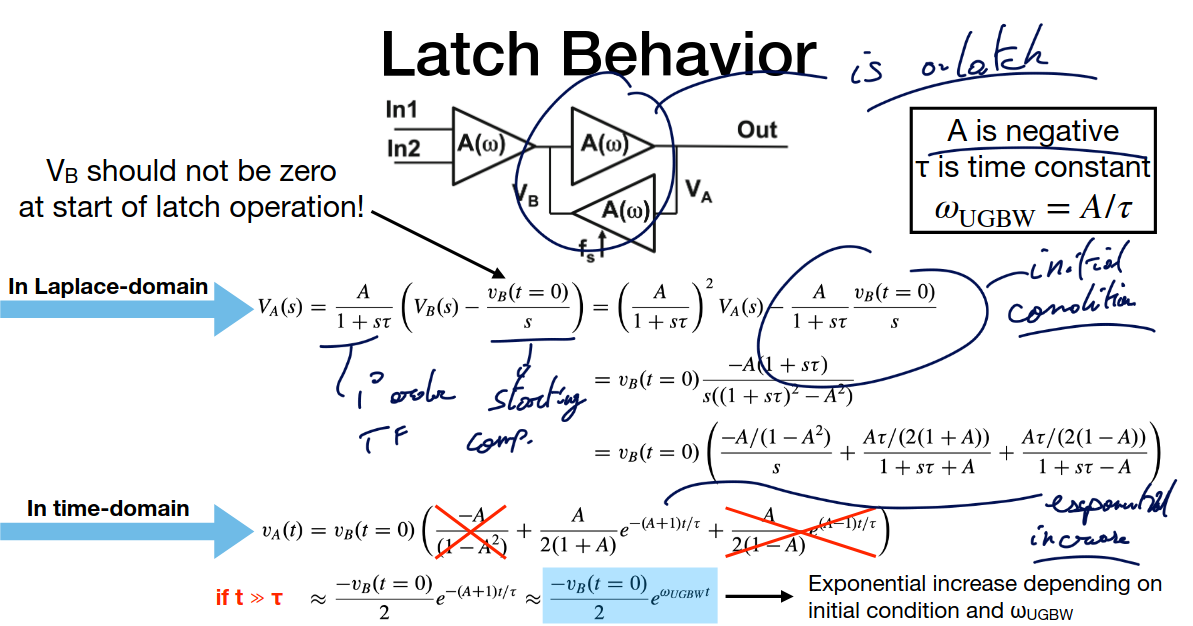
\includegraphics{latch_behavior.png}
\caption{Latch behavior}\label{fig:enter-label}
}
\end{figure}

\hypertarget{non-idealities-1}{%
\subsubsection{Non-idealities}\label{non-idealities-1}}

\hypertarget{comparator-circuit-examples}{%
\subsubsection{Comparator circuit
examples}\label{comparator-circuit-examples}}

\hypertarget{analog-to-digital-converter-topologies}{%
\subsection{Analog-to-digital converter
topologies}\label{analog-to-digital-converter-topologies}}

\hypertarget{conclusions}{%
\subsection{Conclusions}\label{conclusions}}

\hypertarget{delta-sigma-adc}{%
\section{\texorpdfstring{Delta Sigma
{adc}}{Delta Sigma adc}}\label{delta-sigma-adc}}

\hypertarget{basic-principles}{%
\subsection{Basic principles}\label{basic-principles}}

\hypertarget{tab:my_label}{}
\begin{longtable}[]{@{}cl@{}}
\caption{Quick recap of definitions}\tabularnewline
\toprule\noalign{}
Term & Definition \\
\midrule\noalign{}
\endfirsthead
\toprule\noalign{}
Term & Definition \\
\midrule\noalign{}
\endhead
\bottomrule\noalign{}
\endlastfoot
Input sampling rate & Frequency at which the analog input is sampled \\
Output data rate & Frequency at which updated output words are
available \\
Conversion gain & Ratio of an output amplitude over the input
amplitude \\
Bandwidth & Frequency span in which the amplitude of an output sine is
less then 3dB lower as the input amplitude, given a 1:1 conversion
gain \\
{snr} & // \\
{enob} & Error free signal resolution
\(=(SNDR-1.76\text{ dB})/(6.02 \text{ dB})\) \\
\end{longtable}

All those values are important metric when specifying an {adc} but they
can be misleading. We can trick the reader that we achieved exceptional
result with a mediocre implementation. In fact We could find a hugeeee
{snr} if we filter the noise at the input 5 times lower than the nyquist
frequency and then claim a figure that is \(\sqrt{5}\) better than what
we would truly have.

\hypertarget{fom}{%
\subsubsection{\texorpdfstring{{fom}}{fom}}\label{fom}}

There is two main type of {fom} used for {adc} :

\begin{enumerate}
\def\labelenumi{\arabic{enumi}.}
\item
  \ul{Schreier :} It is based on a theoretical idea and on information
  theory. We have a signal power and a maximum efficiency. It is based
  on the \emph{fundamental tradeoff} between accuracy and bandwidth,
  noise and power. But a critique that can be made is the fact it only
  uses {snr} and not the {sndr} which take into account more realistic
  issue.
\item
  \ul{Walden :} It takes into account the {sndr} and also use the
  bandwidth instead of only using the Nyquist frequency. So a more band
  limited {fom}. The {fom} is in Joule per conversion step.
\end{enumerate}

\[\begin{aligned}
        P_{sig,min} &= 8kT \cdot BW \cdot SNR & \text{Power efficiency} &= \frac{P_{circuit}}{P_{sig,min}} = \frac{P_{circuit}}{8kT \cdot BW \cdot SNR}\\
        FoM &= 10^{10} log\left( \frac{SNR\cdot BW}{P_{ADC}} \right) & &=SNR (dB) + 10^{10} log\left( \frac{BW}{P_{ADC}} \right)
\end{aligned}\]

\[\begin{aligned}
            FoM &= \frac{Power}{2^{ENOB} \cdot min(2BW,f_s)}
\end{aligned}\]

There is also an issue related to the actual power consumption. In most
paper, they are only taking into account the power at the input and not
of the full system. In a SAR {adc} for example, \(V_{in}\) will just
control some switches but not directly charge or discharge the cap. SAR
ADC are not that power efficient after all if we take into account the
external bench power supply that is required to let this ADC run.

\hypertarget{signal-conditioning}{%
\paragraph{Signal conditioning}\label{signal-conditioning}}

Again from information theory, we can derive a relation with a
technological constant \(C_T\).

\[\frac{speed (accuracy)^2}{power} = C_T\]

\hypertarget{resolution}{%
\subsubsection{Resolution}\label{resolution}}

The resolution is the \emph{smallest discrete step} a system can take.
Watch out ! resolution \(\neq\) accuracy. We can have a granularity of
16 bits but being unable to provide 16 bits of information (2 bits tied
to ground, ...).

\[resolution = \frac{\Delta I_R}{I_{max} - I_{min}} \cdot 100 \%\]

\begin{figure}
\hypertarget{fig:conversion-chain-label}{%
\centering
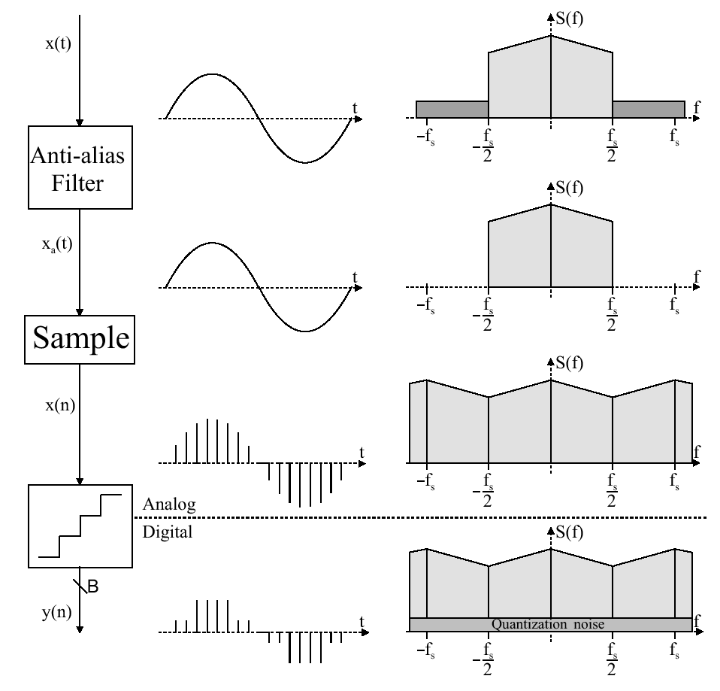
\includegraphics{conversion_chain.png}
\caption{The conversion chain}\label{fig:conversion-chain-label}
}
\end{figure}

We first remove the alias, then sample it to go into discrete time. We
then quantize sampled data which will inevitably introduce quantization
error. Finally to reconstruct we will use a \emph{decimation filter}. In
a Sigma-delta {adc} we will use something called the {osr} to improve
this quantization noise.

\[OSR = \frac{\text{sampling freq } f_s}{\text{Nyquist freq } 2 f_m}\]

For the \(n-\)bit quantizer, it will introduce this infamous quantizer
error that have a seesaw patern up until the overload area where it can
no longer sample anything. This error is :

\[\begin{aligned}
    |V_{in}| &< x_{max} \quad |Q error| < \frac{\Delta}{2} & |V_{in}| &> x_{max} \quad \text{overload}
\end{aligned}\]

The quantization noise is a purely \emph{mathematical model}, it is not
stochastic over time. It represents this transformation of a random
input signal into a random output error due to quantization.\\
We can do the white noise approximation for fast varying signal where
the error is evenly distributed between \([-\Delta/2;\Delta/2]\) with a
pdf value of \(1/\Delta\). We need no overload and need a change in
input.

\[\begin{aligned}
    E(e_q) &= \frac{1}{\Delta I_R} \int_{-\frac{\Delta I_R}{2}}^{\frac{\Delta I_R}{2}} e de = 0 & \sigma_q^2&= \frac{1}{\Delta I_R} E((e_q-E(e_q))^2)\\
    & & &=\frac{1}{\Delta I_R} \int_{-\frac{\Delta I_R}{2}}^{\frac{\Delta I_R}{2}} e^2 de\\
    & & &= \frac{\Delta^2 I_R}{12}
\end{aligned}\]

The power is the \emph{variance} of the signal, which is equivalent to
integrated noise. We only calculate the noise for a specific band.

\[\begin{aligned}
x_{\max} &= 2^B \frac{\Delta}{2} \frac{1}{k} \\ 
S &= y_{\text{rms}}^2 = (k x_{\text{rms}})^2 = k^2 \frac{x_{\max}^2}{2} \\ 
&= 2^{2B - 3} \Delta^2 \\ 
N &= \frac{\Delta^2}{12} \\ 
\Rightarrow SNR &= \frac{12}{8} 2^{2B} = \frac{3}{2} 2^{2B} = SNR_p = 1.76+6.02 B dB
\end{aligned}\]

By going over the sampling much more often we will spread this noise
leading to better SNR performance.

\[\begin{aligned}
N_q &= \int_{-\frac{f_s}{2}}^{\frac{f_s}{2}} S_e^2(f) |H_e^2(f)| |H_d^2(f)| \, df = \int_{-f_b}^{f_b} h_e^2(f) \, df = \frac{\Delta^2}{12} \frac{2 f_b}{f_s} \\
&= \frac{\Delta^2}{12 \, OSR}
\end{aligned}\]

\[\begin{aligned}
SNR_p &= \frac{3}{2} 2^{2B} OSR & SNR_p &= 1.76 + 6.02 B  + 10 log(OSR) \text{ } dB
\end{aligned}\]

The main idea being delta sigma {adc} is to take advantage of previous
error and to integrate it (PI) to correct and go to better values. The
\emph{delta} modulation comes from measuring the error and subtracting
its output from the input. The storing (integrating in continuous time)
is the principle of the \emph{delta-sigma} modulation.

\begin{figure}
\hypertarget{fig:delta-sigma-label}{%
\centering
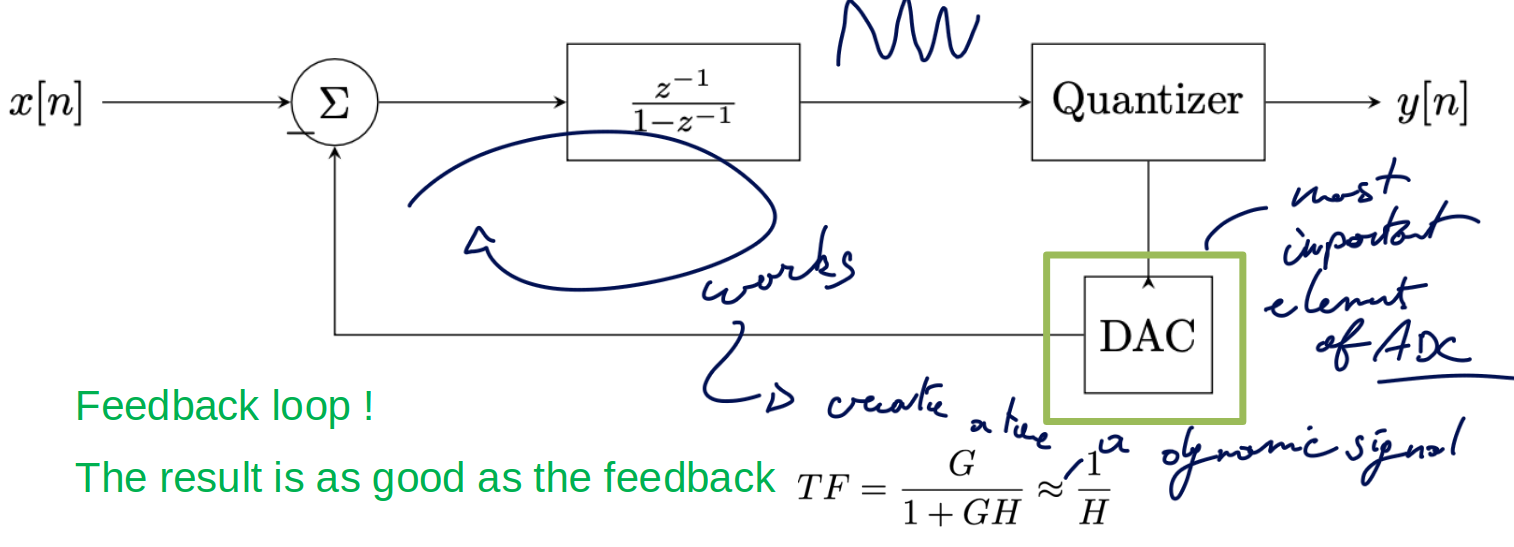
\includegraphics{delta_sigma.png}
\caption{Delta sigma integration}\label{fig:delta-sigma-label}
}
\end{figure}

For the quantizer we can simply go for a comparator so \(1\) or \(-1\)
and this is inherently linear. This will give us a noise and signal
transfer function :

\[\begin{aligned}
STF &= \frac{y}{x} = \frac{G}{1 + GH} & NTF &=  \frac{y}{e} = \frac{1}{1 + GH} \\ 
&= \frac{k \frac{1}{z-1}}{1 + k \frac{1}{z-1}} & &= \frac{1}{1 + k \frac{1}{z-1}}\\ 
&= \frac{k z^{-1}}{1 - z^{-1} + k z-1} & &= \frac{z-1}{z+(k-1)} \\ 
&= z^{-1} \quad \text{for } k = 1
\end{aligned}\]

We can clearly see the different transfer function which is a key aspect
of delta sigma, it will do what we call \emph{noise shaping}. To get the
continuous transfer function we can replace \(z\) by
\(e^{j 2 \pi f/f_s}\). Again to find the SNR we have :

\[\begin{aligned}
    N_Q &= \int_{-f_b}^{f_b} \frac{\Delta^2}{12 f_s} NTF^2 df = \frac{\Delta^2}{4} \left(\frac{\pi}{3} \right)^2 \left( \frac{1}{OSR} \right)^3\\
    S &= \frac{\Delta 2^B}{2\sqrt{2}}\\
    SNR_{dB} &= 10 \cdot log(S) - 10 \cdot log(N_Q) = 6.02B-3.41+30\cdot log(OSR)  \label{eq:snr-noise}
\end{aligned}\]

One major approximation that this formula relies on is the
\(sin\left(\frac{2\pi}{OSR}\right) \approx \frac{2\pi}{OSR}\). So that's
why we need high {osr} values or we won't take advantage of this noise
shaping.

\hypertarget{second-order-sigma-delta}{%
\subsubsection{Second order Sigma
Delta}\label{second-order-sigma-delta}}

\begin{figure}
\hypertarget{fig:2-order-label}{%
\centering
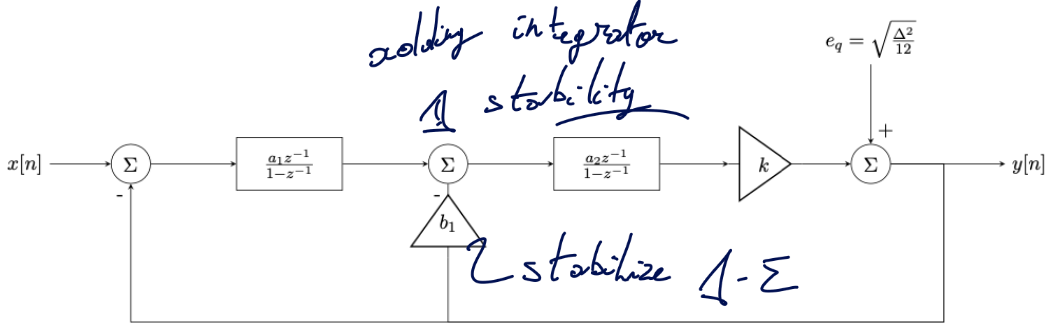
\includegraphics{second_order.png}
\caption{Second order delta sigma}\label{fig:2-order-label}
}
\end{figure}

We can indeed have better noise shaping but we need to take into account
potential instability of this loop. We need to pick the right \(b_1\)
for the job.

\begin{figure}
\hypertarget{fig:equi-2-order-label}{%
\centering
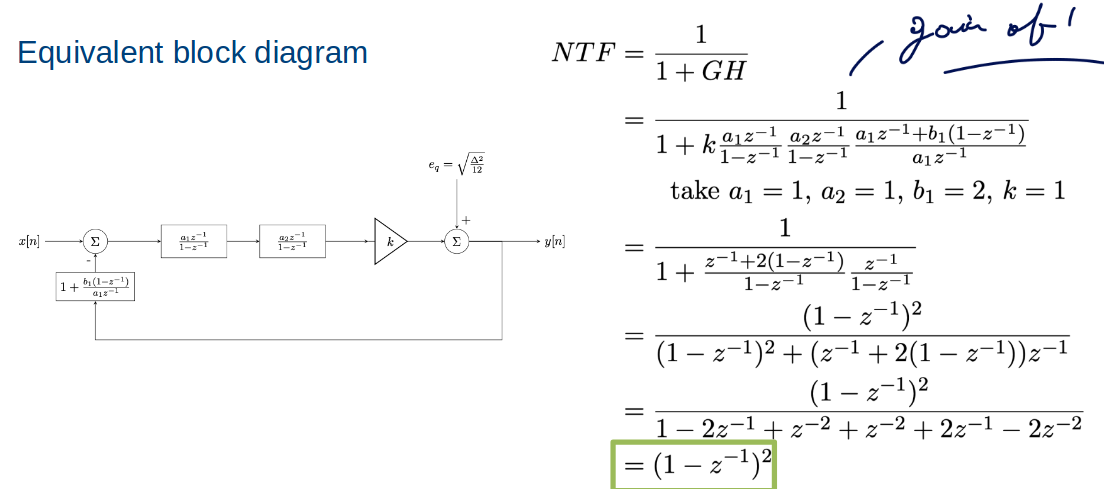
\includegraphics{equi_second_order.png}
\caption{Equivalent second order}\label{fig:equi-2-order-label}
}
\end{figure}

Again, we can reapeat a similar process as in equation
\protect\hyperlink{eq:snr-noise}{{[}eq:snr-noise{]}} and have :

\[\begin{aligned}
    SNR &= 6.02B-11.1 +50\cdot log(OSR)\\
    SNR_n &= 6.02B- 10\cdot log \left( \frac{2\pi^{2n}}{3(2n+1)} \right) +10(2n+1)\cdot log(OSR)
\end{aligned}\]

We can also have other issues that will limit our {enob}, typically we
can have third order distortion. But again, some paper will cheat and
move the \(f_{in}\) as close as the cut-off frequency so the third order
distortion won't be seen.\\
The main action of a delta sigma, is converting a signal into a {pwm}
signal. But we could also face some saturation where the width of the
signal doesn't reflect or mean any information. We need the amplitude to
be lower as the feedback voltage to avoid \emph{overload}. Different
order sigma delta have some different overload criteria, we will try to
spread this swing to avoid overloading early stage integrator.

\hypertarget{stability-and-limit-cycle}{%
\subsubsection{Stability and Limit
Cycle}\label{stability-and-limit-cycle}}

We know it is a feedback system so having the wrong coefficients will
make an instable system. We can witness some \emph{limit cycle} as
starting with some starting condition will evolve with the same
trajectory. The instability can be seen as a loop that will go towards
infinity and won't find stability. Usually, this will be limited by the
supply range.

\hypertarget{pattern-noise}{%
\paragraph{Pattern noise}\label{pattern-noise}}

There is a pattern in the ideal output at \(f_s / 4\) and is called the
limit cycle. Cause of this, the quantization is no longer white and we
cannot longer do noise shaping. Dead zone in DC transfer function. We
can use some matlab models to check for stability.

\textbf{page 51}

\[\nabla \times \left( \frac{1}{\mu} (\nabla \times \mathbf{A}) \right) = \mathbf{J} + \epsilon \frac{\partial}{\partial t} \left( -\nabla \Phi - \frac{\partial \mathbf{A}}{\partial t} \right)\]

\end{document}
